\chapter{Shortcuts to calculate objects in General Relativity}
This chapter will address calculations in General Relativity. GR contains many important expressions that are required to be calculated but the sheer number of indices can often be a barrier in detangling the values of these expressions. We work through some examples and explain the importance of developing a technique in calculations. 

We are almost always given a metric ansatz $g_{\mu\nu}(x)$. From this initial metric, we can work calculate basically every piece of information about the dynamics on our manifold. The following cascade will help to understand, 
\begin{equation}    
\end{equation}

Following this cascade, will help us to determine the curvature side of the Einstein Field Equations, $G_{\mu\nu} = 8\pi GT_{\mu\nu}$
\section{Christoffel Symbols}
The most basic quantity we can calculate, given a metric, are the Christoffel symbols. At the face of it, $\Gamma^{\alpha}_{\ \mu\nu}$ has three indices each of which can range from $\{0,1,2,3\}$. So, in a $d$-dimensional spacetime (1 timelike dimension and $(d-1)$ spacelike dimensions) that's at most, $d^3\ (=64\text{ in }d=4\text{-spacetime})$ non-zero components to calculate. However, we note that that Christoffel symbols are symmetric under the exchange of the two covector indices, $\Gamma^{\rho}_{\ \mu\nu} = \Gamma^{\rho}_{(\mu\nu)}$, which means we can eliminate some of these possibilities. Taking this into consideration, we now have at most $2d(d+1)$ non-zero terms to calculate, which is a little bit better ($d^3\geq 2d(d+1)$).
\subsection{Calculating the Christoffel Symbols}
We can imagine the Christoffel symbols as a $d$-paged booklet, with each page labelled by $\rho = \{0, 1, 2, 3\}$. Each page contains a $(d\times d)$-matrix. 

\begin{figure}
\centering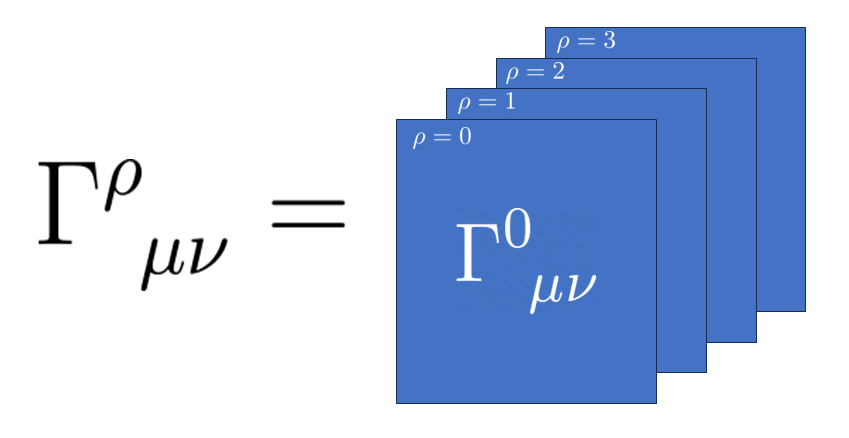
\includegraphics[width=0.75\textwidth]{Images/gammaBooklet.PNG}
\caption{\footnotesize{Each page of this book is a matrix labelled by the value of $\rho$.}}
\label{fig:gamma-booklet}
\end{figure}

This is more instructive through examples. 
\subsubsection{Example: Metric on a $S^2$}
We will initially work on calculating the Christoffel symbols on a unit two-sphere, $S^2$ ($d=2$). The metric is given by, 
\begin{equation}\label{two-sphere-metric}
    \d s^2 = \d\theta^2 + \sin^2(\theta)\d\phi^2,
\end{equation}
and so we can already note that, $g_{\theta\theta} = 1$ and $g_{\phi\phi}=\sin^2(\theta)$ (note: $\theta$ and $\phi$ are not Lorentz indices, but are labels for the corresponding coordinates in the metric). There are only two \textit{pages} in this set of Christoffel symbols, $\Gamma^{\theta}_{\ ij}$ and $\Gamma^{\phi}_{\ ij}$ 
\begin{equation}
\begin{split}
\Gamma^{\theta}_{\ ij} &= \frac{1}{2}g^{\theta k}\left(g_{ik,j} + g_{jk,i} - g_{ij,k}\right)\\
\Gamma^{\phi}_{\ ij} &= \frac{1}{2}g^{\phi k}\left(g_{ik,j} + g_{jk,i} - g_{ij,k}\right)
\end{split}
\end{equation}
An additional note on the structure of these expressions, the metric is purely diagonal, therefore there is an additional constraint placed on the index $k$, in that it has to match the other index on the $g^{\mu\nu}$ factor\footnote{This will almost always be the case as we will deal with only diagonal metrics.}. Also we can drop terms containing derivatives of $\phi$ because it is an \textit{ignorable coordinate} ($g$ is not an explicit function of $\phi$), 
\begin{equation}
    \begin{split}
        \Gamma^{\theta}_{\ ij} &= \frac{1}{2}\left(g_{i\theta,j} + g_{j\theta,i} - g_{ij,\theta}\right)\\
\Gamma^{\phi}_{\ ij} &= \frac{1}{2\sin^2\theta}\left(g_{i\phi,j} + g_{j\phi,i}\right).
    \end{split}
\end{equation}
This is still completely general for all symbols in this example. Now we can choose all possible combinations of the coordinates, which is easy in this example because there's only two coordinates. Terms proportional to any derivatives of $g_{\theta\theta}$ will vanish, 
\begin{eqnarray*}
    \Gamma^{\theta}_{\ \theta\theta} &=& \Gamma^{\theta}_{\ \theta\phi}=0, \ \ \ \ \Gamma^{\theta}_{\ \phi\phi} = -\frac{1}{2}g_{\phi\phi,\theta} = -\frac{1}{2}\frac{\partial}{\partial\theta}(\sin^2\theta) = -\sin\theta\cos\theta\\
    \Gamma^{\phi}_{\ \theta\theta} &=& \Gamma^{\phi}_{\ \phi\phi} = 0,\ \ \ \ \Gamma^{\phi}_{\ \theta\phi} = \frac{1}{2\sin^2\theta}\frac{\partial}{\partial\theta}g_{\phi\phi} = \frac{1}{2\sin^2\theta}(2\sin\theta\cos\theta) = \cot\theta.
\end{eqnarray*}
In matrix form, we can write the following, 
\begin{equation}
\Gamma^{\theta}_{\ ij} = 
\begin{pmatrix}
    0 & 0 \\
    0 & -\sin\theta\cos\theta
\end{pmatrix}_{ij}\ \ \ \ \ \
\Gamma^{\phi}_{\ ij} = 
\begin{pmatrix}
    0 & \cot\theta \\
    \cot\theta & 0
\end{pmatrix}_{ij}.
\end{equation}
Although this was a simple example, using this method becomes more efficient for keeping track of indices in higher-dimensional examples and facilitates a neater calculation. 
\subsubsection{Metric on a surface of constant proper time embedded in $\mathbb{M}^{1,3}$}
Consider the Minkowski spacetime in inertial coordinates, $x^{\mu}$. Consider the three-dimensional surface of points that can be reached in proper time $R$, where $R\geq 0$. The surface is given by the equation, 
\begin{equation}\label{surface of constant tau}
    R^2 = t^2 - (x^2 + y^2 + z^2)
\end{equation}
This surface can be parametrised by the following coordinate transformation, 
\begin{equation}
    \begin{split}
        t = R\cosh\xi,\ \ 
        z = R\sinh\xi\cos\theta,\ \ 
        y = R\sinh\xi\sin\theta\sin\phi,\ \
        x = R\sinh\xi\sin\theta\cos\phi,\ \ 
    \end{split}
\end{equation}
with $\xi\in(0,+\infty]$, $\theta\in[0, \pi)$ and $\phi\in(0,2\pi]$. By change of coordinates, the metric can be found to be. Under a general coordinate transformation, we know that the metric components transform as, 
\begin{equation}
    g_{\mu'\nu'}(x') = \frac{\partial x^{\mu}}{\partial x^{'\mu'}}\frac{\partial x^{\nu}}{\partial x^{'\nu'}}g_{\mu\nu}(x),
\end{equation}
where $x^{\mu} = (t,x,y,z)$ and $x^{'\mu'} = (\xi, \theta,\phi)$ (we have one less coordinate in the new frame because the dependence (\ref{surface of constant tau}) removes one of the degrees of freedom). If we recall that the metric is a diagonal matrix, the only surviving terms on the right-hand side have $\mu = \nu$. So we are then free to choose the $\mu'$ and $\nu'$ indices. Look at the $g_{\xi\xi}$ term and notice that each component of $x^{\mu}$ depends on $\xi$, 
\begin{equation}
    \begin{split}
        g_{\xi\xi} &= \frac{\partial x^{\mu}}{\partial\xi}\frac{\partial x^{\nu}}{\partial \xi}g_{\mu\nu}(x) \\
        &= -\left(\frac{\partial t}{\partial\xi}\right)^2 + \left(\frac{\partial x}{\partial\xi}\right)^2 +  
        \left(\frac{\partial y}{\partial\xi}\right)^2 +   
        \left(\frac{\partial z}{\partial\xi}\right)^2\\
        &= R^2\left[-(\sinh\xi)^2 + (\cosh\xi\cos\theta)^2+(\cosh\xi\sin\theta\sin\phi)^2 + (\cosh\xi\sin\theta\cos\phi)^2\right]\\
        &=R^2.
    \end{split}
\end{equation}
Following along the same lines, we find the metric, 
\begin{equation}
    \d s^2 = R^2\left[\d\xi^2 + \sinh^2\xi(\d\theta^2 + \sin^2\theta\d\phi^2)\right]
\end{equation}
This is the line element on a three-dimensional hyperbolic space, $\mathbb{H}^3$. Now, the Christoffel symbols of this metric (note that $\phi$ is ignorable, so any derivatives with respect to $\phi$ will vanish), 
\begin{equation}
    \begin{split}
  \Gamma^{\xi}_{\ ij} &= \frac{1}{2R^2}\left(g_{i\xi,j} + g_{j\xi,i} - g_{ij,\xi}\right)\\
  \\
    \Gamma^{\xi}_{\ \xi\xi} &= \Gamma^{\xi}_{\ \xi\theta} = \Gamma^{\xi}_{\ \xi\phi} = \Gamma^{\xi}_{\ \theta\phi} = 0,\\
    \Gamma^{\xi}_{\ \theta\theta} &= -\sinh\xi\cosh\xi,\\
    \Gamma^{\xi}_{\ \phi\phi} &= -\sinh\xi\cosh\xi\sin^2\theta\\
\end{split}
  \end{equation}
  
\begin{equation}
\begin{split}
\Gamma^{\phi}_{\ ij} &= \frac{1}{2R^2\sinh^2\xi}\left(g_{i\theta,j} + g_{j\theta,i} - g_{ij,\theta}\right)\\
\\
    \Gamma^{\theta}_{\ \xi\xi} &= \Gamma^{\theta}_{\ \xi\phi} = \Gamma^{\theta}_{\ \theta\theta} = \Gamma^{\theta}_{\ \theta\phi}=0\\
    \Gamma^{\theta}_{\ \xi\theta} &= -\sin^2\theta\coth\xi\\
    \Gamma^{\theta}_{\ \phi\phi} &= -\sin\theta\cos\theta.
\end{split}
\end{equation}


\begin{equation}
\begin{split}
\Gamma^{\phi}_{\ ij} &= \frac{1}{2R^2\sinh^2\xi\sin^2\theta}\left(g_{i\phi,j} + g_{j\phi,i}\right)\\
\\
    \Gamma^{\phi}_{\ \xi\xi} &= \Gamma^{\phi}_{\ \xi\theta} = \Gamma^{\phi}_{\ \theta\theta} = \Gamma^{\phi}_{\ \phi\phi} =0\\
    \Gamma^{\phi}_{\ \theta\phi} &= \cot\theta\\
    \Gamma^{\phi}_{\ \xi\phi} &= \coth\xi
    \end{split}
\end{equation}
We can write these in the following matrix form, 
\begin{equation}
\begin{split}
\Gamma^{\xi}_{\ ij} &= 
\begin{pmatrix}
    0 & 0 & 0\\
    0 & -\sinh\xi\cosh\xi & 0\\
    0 & 0 & -\sinh\xi\cosh\xi\sin^2\theta
\end{pmatrix}_{ij}\\
\Gamma^{\theta}_{\ ij} &= 
\begin{pmatrix}
    0 & -\sin^2\theta\coth\xi & 0\\
    -\sin^2\theta\coth\xi & 0 & 0\\
    0 & 0 & -\sin\theta\cos\theta
\end{pmatrix}_{ij}\\
\Gamma^{\phi}_{\ ij} &= 
\begin{pmatrix}
    0 & 0 & \cot\theta\\
    0 & 0 & \coth\xi\\
    \cot\theta &\coth\xi & 0
    \end{pmatrix}_{ij}.
\end{split}
\end{equation}
\subsubsection{Christoffel symbols of the Schwarzschild  Metric}
Consider the metric of static, two-sphere of mass $M$, with Schwarzschild radius, $r_S = 2GM$,
\begin{equation}
    \d s^2 = -(1-r_S/r)\d t^2 + (1-r_S/r)^{-1}\d r^2 + r^2\d\Omega^2
\end{equation}
where $\d\Omega^2$ is the metric on a two-sphere as in (\ref{two-sphere-metric}).
The Christoffel symbols for a static solution are,  
\begin{equation}
    \begin{split}
        \Gamma^{t}_{\ ij} &= -\frac{r}{2(r-r_S)}\left(g_{it,j} + g_{jt,i}\right) 
    \end{split}
\end{equation}
But the only non-vanishing component of this matrix is, 
\begin{equation}
    \Gamma^{t}_{\ tr} = \frac{r_S}{2r(r-r_S)} 
\end{equation}
Now we move on to the other components
\begin{equation}
\begin{split}
    \Gamma^{r}_{\ ij} &= \frac{r-r_S}{2r}\left(g_{ir,j} + g_{jr,i} - g_{ij,r}\right)\\ 
    &=
    \begin{pmatrix}
        -\frac{r_S(r-r_S)}{2r^3} & 0 & 0 & 0 \\
        0 & -\frac{r_S}{2r(r-r_S)} & 0 & 0 \\
        0 & 0 & (r_S-r) & 0 \\
        0 & 0 & 0 & (r_S-r)\sin^2\theta 
    \end{pmatrix}
\end{split}
\end{equation}
Not the $\theta$ matrix,
\begin{equation}
    \Gamma^{\theta}_{\ ij} = \frac{1}{2r^2}\left(g_{i\theta,j} + g_{j\theta,i} - g_{ij,\theta}\right) = 
    \begin{pmatrix}
        0 & 0 & 0 & 0 \\
        0 & 0 & r^{-1} & 0 \\
        0 & r^{-1} & 0 & 0 \\
        0 & 0 & 0 & -\sin\theta\cos\theta
    \end{pmatrix}
\end{equation}
Which leaves $\phi$,
\begin{eqnarray}
    \Gamma^{\phi}_{\ ij} = \frac{1}{2r^2\sin^2\theta}\left(g_{i\phi,j} + g_{j\phi,i} - g_{ij,\phi}\right)= 
    \begin{pmatrix}
        0 & 0 & 0 & 0 \\
        0 & 0 & 0 & r^{-1} \\
        0 & 0 & 0 & \cot\theta  \\
        0 & r^{-1} & \cot\theta & 0
    \end{pmatrix}
\end{eqnarray}

